\documentclass[main.tex]{subfiles}

\begin{document}

 \notinmain{ka ble ikke gjort/kva må bli gjort i fremdtiden, hvordan kan system bli gjenbrukt til readout electronics og cooling}

\section{Discussion}
\textit{This chapter describes the functionality of the control software created in this thesis, what is complete and what is missing. The chapter covers missing features and how the software can be expanded in the future. A discussion is also made on the modularity of the system and how the system can be repurposed within the PCT project.}

\subsection{Future work}

The control software presented in this thesis is not complete, due to time limitations and because the system it is interfacing is not complete. This section will go over work that needs to be done for the control software.


\subsection{Error handling}

\subsubsection{Control Software}

The error handling from the control software is not finalized. By "errors", we are referring to the error messages from the microcontroller, which is discussed in \autoref{ssec: microcontroller}. Currently, only the monitoring system checks for errors during its polling function. The design of the error handling has not been decided yet, but this section will go over potential implementations.

Both the configuration system and the monitoring system requires functions to retrieve errors and process them. This suggests that an "Error Manager" class should be developed, which contains general functions for handling the errors. Both the configuration and monitoring \gls{api}s could use this manager to handle errors, which would reduce redundant code in the \gls{api}s, as well as increase the modularity of the software.

A design choice must be made on how to store and display the errors from the microcontroller. Ideally, the error messages should be stored in a logging database, and displayed to the user, but which database to use, and how to display it have not been decided yet. Currently, the error messages is not stored, only displayed in the monitoring \gls{gui}. InfluxDB could be used to store logging information, and separate tags could be made to indicate the severity of each error. Another option for handling logging is Grafana Loki, a log aggregation system which is optimized for Grafana. 

\subsubsection{microcontroller}
The microcontroller software supports custom control functions that can be performed by writing to the control registers on the microcontroller. Utilizing these custom functions could reduce the number of transmissions needed for error handling, increasing the speed of the error handling algorithm. For example, identifying faulty strings would be a cumbersome process for the control software; turning on the strings to test their current consumption individually would require multiple transmissions through the entire \gls{pcs}-chain. A microcontroller function that automatically turns each stave on, one by one, and then measures their current consumption would make the process significantly faster. The control software would only need to call the function by writing to a register, retrieve the current values for each string, and compare them to the expected ones.

\subsection{Configuration System}

Currently, the broadcast function in the MB Hub is not used in the configuration process. This is due to the structure of the database is set to have a value for every configuration register on every layer. Using the broadcast functionality would require a separate function that checks if a register value is the same for every layer, and if yes, broadcast the data, if not, it would have to configure the layers separately. This would not only be cumbersome work, but it could potentially add more delay in the form of software overhead.

It is required to restructure the database to be able to effectively use the broadcast function. A possible solution is the use of a "default" configuration set in the database. We would by default have a configuration set that is used to configure all layers, but have exception lists for layers that require different values for certain registers. The default set is merged with the exception values and create the final configuration set. A figure of the possible implementation of a default configuration set is given in \autoref{fig: default_database}.

\begin{figure}[!ht]
    \centering
    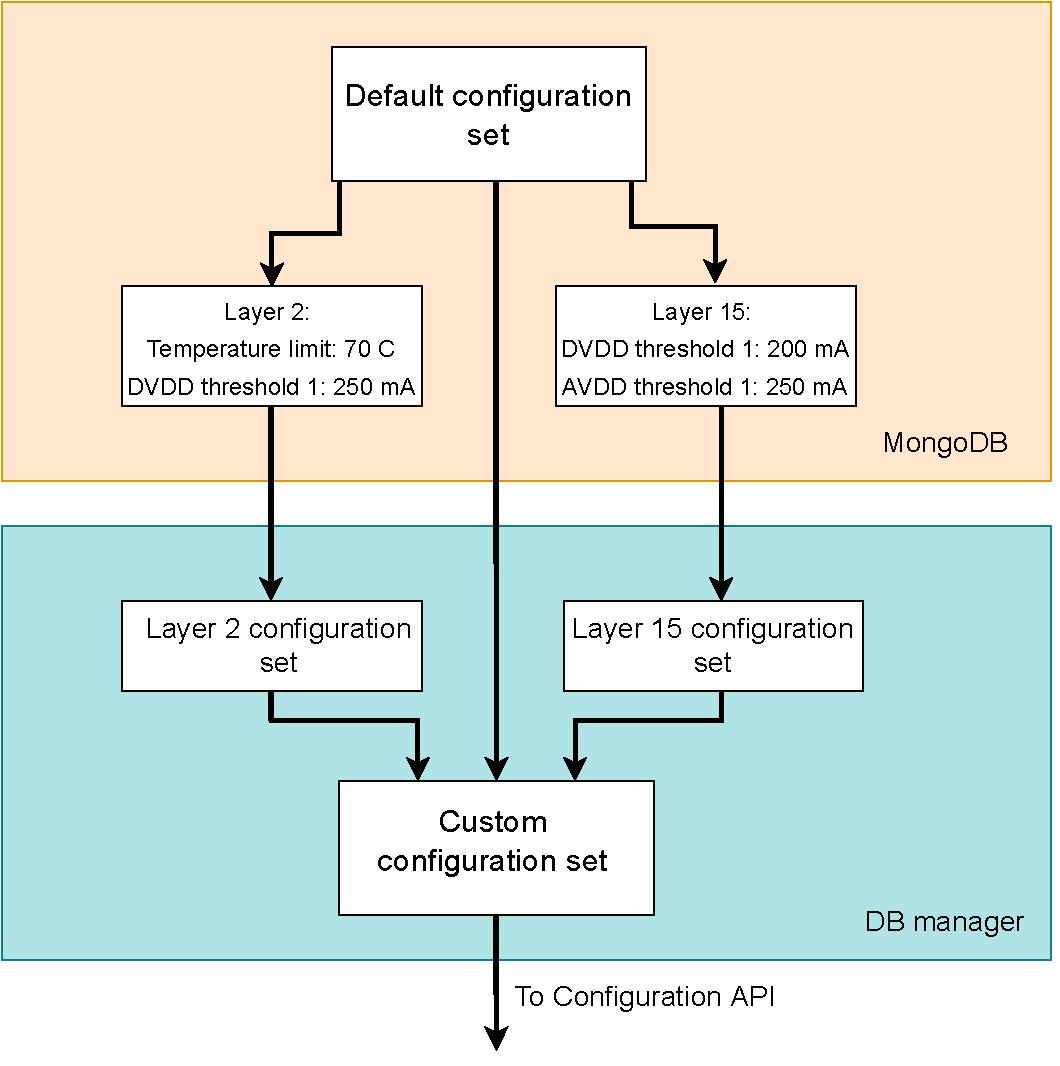
\includegraphics[scale=0.55]{images/default_database.pdf}
    \caption{Block diagram showing the implementation of a "default" configuration set in MongoDB.}
    \label{fig: default_database}
\end{figure}
\FloatBarrier 

The figure shows the default configuration set in the MongoDB database, exception lists for two layers, and the DB manager class retrieves the configuration set. DB manager will create a configuration set for each layer with an exception list and merge this configuration set with the default one, which gives us a custom configuration set. This custom set is then sent to the configuration \gls{api}. Restructuring the database like this would also require changing the configuration \gls{api} to utilize the broadcast function.

The calculations and results from \autoref{ssec: con_timing} show that the configuration timing is already adequate for this project, only spending half a second to configure all layers. The default database presented in this section could be implemented in the future if timing becomes a problem.

\subsection{Grafana}

The Grafana dashboard has four tabs for each measurement type: DVDD, AVDD, PWELL, and temperature. Each tab contains histograms for each layer, but it is currently impossible to display all tabs on one screen; this design may be cumbersome for the user. They must scroll through the tabs if they want to view multiple measurements simultaneously.

If the Grafana design is not satisfactory to the user in the future, a new dashboard design is warranted. A group of users should create this new design to ensure the dashboard is user-friendly.


 
 \subsection{Docker Image}
 
 The control system uses several different packages and programs to function. The README-file in the GitHub repository gives instructions on how to install all dependencies and run the program, but it is still cumbersome to move the system to a different computer. Therefore, in future work, a Docker Image of the system should be created. Docker is a program that allows for building an "Image", which is a virtual environment for your program, containing all dependencies necessary to run the program. By building a Docker Image of your program, moving it to other computers only requires downloading a single docker file and running it.
 
 The main hub \gls{gui}, along with its lower level \gls{gui}s and \gls{api}s can all be encapsulated in one Docker Image. The databases and Grafana will most likely be located on different servers, therefore each of them should have their own Docker Image with their ports open to the \gls{gui} Image.
 
 \subsection{Reusability}
 
 The configuration and monitoring systems developed in this thesis have been built using software design standards to make it generic and modular. The system is layered in such a manner that individual parts with specific functions can be reused in other systems. This section discusses how these parts can be reused.
 
 \subsubsection{Monitoring software}
The monitoring software is comprised of \textit{influx\_api}, \textit{configuration\_api}, and \textit{panda\_filter}. The influx api class requires very little modification to be used in other systems. The \gls{api} has functions for inserting values into the database, and for filtering data points with the \textit{panda\_filter} class. Certain tags in the class must be redefined to match the new system it interfaces with, i.e. change "layer" to "flowmeter", for example.

The panda filter class uses pandaframe to filter received data. It currently is only capable to filter data based on the exception process described in \autoref{ssec: downsampling}, but additional functions can be created to perform other filters on the data.

The monitoring \gls{api} does not require any direct modification to be repurposed to another system, but it requires a lower level \gls{api} to interface with, akin to the microcontroller \gls{api}. The \textit{monitor\_addr} list must also be edited to include the desired registers to poll.

\subsubsection{Configuration software}

The configuration software is comprised of \textit{db\_manager}, and \textit{configuration\_api}. The configuration \gls{api} is specialized to configure, and power on the \gls{pcs}; the configuration functions must therefore be reworked for other systems. \autoref{ssec: power_algo} shows that the configuration process is in two stages, stage 1 configures general registers, and stage 2 performs the ramp-up algorithm. Stage 1 may be suitable to reuse since it only performs basic write operations. However, stage 1 also contains system-specific functions, such as handshake verification, that must be removed or modified.

The \textit{db\_manager} is the interface between the Python classes and MongoDB. It is relatively simple; its primary function is to create configuration sets for the \gls{pcs}. The configuration sets store single values for most registers, but the threshold 2 registers have individual values for each string. This formatting must be revised or removed if we reuse the manager to create configuration sets in the future. 

The lower level \gls{api}s that connect to the microcontroller and the MB Hub uses IPbus to communicate, and other systems that uses IPbus can base their design on these \gls{api}s. The readout system in particular, uses IPbus for configuring the ALPIDE-sensors, and therefore could base its structure on the Power Control System \gls{api}. The cooling system reads out data using Moxa modules, not IPbus, which means the lower level \gls{api} must be redefined, but it could still utilize the same concepts, such as having multiple levels of \gls{api} abstraction.
 
 \subsubsection{Register Package}
 
The \gls{api}s developed for the \gls{pcs} use namedtuples to process register information, which is described in \autoref{ssec: mcu_api}. The namedtuples make it easier to repurpose the \gls{api}s to a different system. A developer can define the address map of a different module using the same namedtuples, and the \gls{api}s would only require small modifications to work with the new system.
 
\subsection{USART communication}

The communication link between the MB Hub and the microcontroller is outside the scope of this thesis. However, significant time have been spent on creating verification tests of the \gls{pcs}, and this by extension, includes the USART communication between the MB Hub and the microcontroller. This section covers the potential sources of these errors.

A 17 hour test was done on the USART communication in an earlier part of the development cycle, and no errors were observed. There were however errors observed at lower baud rates. The test setup was then briefly moved to an expo, and after returning, the error rate was observed to be much higher, similar to the results shown in \autoref{ssec: bit_error}, even at higher baud rates. These results suggests there exist two sources of errors in the communication, the first is dependent on the baud rate of the \gls{usart}, and the other is most likely caused by the inconsistent test environment. \notinmain{Skriv her mer om hva potensiellt er årasken til feilene etter at eg har omskrevet test kapittelet. Altså delta tid i baud rates og uneven ground levels.}

Previous tests of the prototype did not suffer from any errors in the bit, and as such the most probable cause of the errors is due to inconsistent test environment. Due to time constraints, further tests and troubleshooting were not done, but the underlying issue most likely comes from uneven ground levels between \gls{fpga} and microcontroller, since the bit flip is always a zero turning into a one, never the other way.

\end{document}